 

%\documentclass{article}
\documentclass[11pt]{article}
\usepackage{amssymb,latexsym}
\usepackage[turkish]{babel}
\usepackage{amsmath, amsthm, amssymb, amsfonts, mathrsfs}
\usepackage[utf8]{inputenc}
\usepackage{relsize}
\usepackage{tikz}
\usepackage{graphicx}
\usepackage[T1]{fontenc}
\usepackage{lmodern}
\usepackage{tikz}
\usetikzlibrary{calc,trees,positioning,arrows,chains,shapes.geometric,%
  decorations.pathreplacing,decorations.pathmorphing,shapes,%
  matrix,shapes.symbols}
\usetikzlibrary{decorations.pathmorphing,shadows} 
\usepackage{xcolor}
\usepackage{mathtools}
\theoremstyle{plain}
\newtheorem{theorem}{Teorem}
\newtheorem{corollary}{Sonuç}
\newtheorem*{main}{Ana Teorem}
\newtheorem{lemma}{Yardımcı Teorem}
\newtheorem{proposition}{Önerme}
\newtheorem{example}{Örnek}
\newtheorem{remark}{Uyarı}

\theoremstyle{definition}
\newtheorem{definition}{Tanım}

\theoremstyle{remark}
\newtheorem*{notation}{Notasyon}

\numberwithin{equation}{section}
\renewcommand{\%}{{\small \%}}
\begin{document}
%\title[Topolojik Vektör Uzayları]
    %  {Topolojik Vektör Uzayları}
\title{\bfseries { Topolojik Vektör Uzayları}}
\date{\vspace{-5ex}}
%\author{ Kaya Ademoğulları}

%\address{Computer Science Department\\
 %        University of Winnebago\\
 %        Winnebago, Minnesota 53714} 
%\email{menuhin@ccw.uwinnebago.edu}
%\urladdr{http://math.uwinnebago.ca/homepages/menuhin/}
%\thanks{Research supported by the NSF under grant number
%~23466.}  
%\keywords{topolojik uzaylar, vektör uzayları,
%ağlar} 
%\subjclass{Primary: 06B10; Secondary: 06D05}
%\date{27 Kasım 2013}
%\begin{abstract}
 %  In this note we prove that there exist \emph{complete-simple distributive
 %  lattices,} that is, complete distributive lattices in which there are 
 %  only two complete congruences. 
%\end{abstract}

\maketitle

\section{Vektör Uzayları}\label{S:intro} 
%Bu bölümde kısaca topolojik uzaylar hakkında fazla detaylı olmayan hatırlatmalar yapılacaktır.

Reel yada komlex sayılar cismi üzerine bir vektör uzayı, aslında üç boyutlu sıradan bir Öklid Uzayının doğal bir genelleştirilmiş halidir. Burada iki cebirsel işlem var, vektörlerin toplanması ve bir vektörün bir skalerle çarpımı. Bunların birtakım mantıklı koşulları karşılamaları gerekiyor. $\Phi$ cismi üzerine tanımlı bir $E$ vektör uzayı alalım. Bu iki işlem, vektörlerin toplanması ve bir vektörün bir skalerle çarpımı, $x,y\in E$ \text{için} $x+y\in E$, $\forall x\in E $ ve $\lambda\in \Phi$ için $\lambda x\in E$ olacak şekilde tanımlı olsun.
\begin{enumerate}

\item \quad $x+y=y+x$ 
\item \quad $x+(y+z)=(x+y)+z$
\item \quad $E$'nin bir sıfır elemanı vardır; buna orijin de diyoruz, öyle ki
\[\forall x\in E,\quad 0+x=x\]
\item \quad $\forall x\in E$ bir $-x$ vardır, öyle ki, $x+(-x)=0$
\item \quad $(\lambda\mu)x=\lambda(\mu x)$
\item \quad $\lambda(x+y)=\lambda x+\lambda y$
\item \quad $(\lambda+\mu)x=\lambda x+\mu x$
\item \quad $1.x=x$
\end{enumerate}
Bunlardan sıfırın ve $\forall x\in E$ için $-x$ sayısının biricikliğini anlıyoruz. Böylece $E$'deki her $x$ elemanı için, $0.x=0$, $(-1).x=-x$ ve $\forall\lambda\in\Phi$ için $\lambda.0=0$ eşitliklerine ulaşmak kolaylaşıyor.\\[2pt]

Belirli bir $P(x)$ özelliğini sağlayan $x$ elemanlarının oluşturduğu kümeyi $\{x:P(x)\}$ şeklinde gösteriyoruz. $E$'nin altkümeleri ve onların elemanları ile ilgili kombinasyonlar hakkında şu şekilde bir notasyon kullanıyoruz:\\[3pt]
$x\in E$ ve $A\subseteq E$ ise, \quad $x+A=\{x+y:y\in A\}$\\[2pt]
$A\subseteq E$ ve $B\subseteq E$ ise, \quad $A+B=\{x+y:x\in A, y\in B\}$\\[2pt]
$\lambda\in\Phi$ ve $A\subseteq E$ ise,\quad $\lambda A=\{\lambda x:x\in A\}$\\[2pt]
Aynı zamanda, $\mathscr{A}$, $E$'nin altkümelerinin bir kümesi olmak üzere, \[x+\mathscr{A}=\{x+A:A\in \mathscr{A}\}\]
Bu arada $A+A\neq2A$ olmakla birlikte, $2A\subseteq A+A$ olmaktadır. \emph{(Neden?)}

$E$ vektör uzayının bir $M$ altkümesinin, \textbf{bir altvektör uzayı} olması için iki şartımız var;
\begin{equation}
M+M\subseteq M 
\end{equation}
ve $\forall\lambda\in\Phi$ için 
\begin{equation} \lambda M\subseteq M
\end{equation}
Bunu, yukarıda da belirttiğimiz gibi, $\forall x,y\in M$ ve $\forall\lambda\in\Phi$ için,
\[
x+y\in M\qquad \lambda x\in M
\]olarak anlamamız gerekiyor.\\[7pt]

\textbf{Örnek} verecek olursak, $\mathbb{R}^2$, $\mathbb{R}$ cismi üzerinde bir vektör uzayı olmak üzere
\[M=\{(x,0):x\in\mathbb{R}\}\]
şeklinde tanımladığımız $M$ kümesi, $\mathbb{R}^2$ nin bir altvektör uzayıdır. $M$'den alacağımız iki elemanın toplamının $M$ kümesine ait olmasının yanısıra bu elemanların $\lambda$ gibi bir skalerle çarpımının da $M$ kümesinde bulunduğunu görürüz.

$\{0\}$ kümesi, ki sadece orijin noktasını eleman olarak kabul eden kümedir, başlıbaşına bir altvektör uzayıdır.\newpage

\emph{\textbf{Altvektör uzaylarının herhangi bir arakesiti de altvektör uzayıdır.}}
\begin{proof}
$E$'nin altvektör uzayları ailesi, $i\in J$ bir indis kümesi olmak üzere $\{M_i\}$ olsun. Bu aileden aldığımız herhangi bir miktarda elemanın arakesitini
\[
M=\bigcap_{i\in J} M_i
\] ile gösterelim. Herhangi bir $ i\in J$ için $m_{1},m_2\in M_i$ aldığımızda, seçeceğimiz bu iki eleman, altvektör uzayı ailesinin her birinin, yani arakesit kümesinin, $M$'nin  elemanlarıdır, $M_i$ altvektör uzayı olduğundan toplamlarının da aynı $M_i$ kümesine ait olduğunu görürüz.  Bu durum $\forall i\in J$ için geçerli olduğundan $m_{1}+m_{2}\in\bigcap_{i\in J} M_i$. O halde, $M+M\subseteq M$\checkmark \\[5pt]
$M$ kümesinden aldığımız bir $m$ elemanı, arakesiti oluşturan bütün altvektör uzaylarının da elemanı olduğu için, ve $\lambda\in\Phi$ için $\lambda m$ yine bu kümelere ait olacağından, arakesitte de bulunacaktır. 
\[
\lambda M=\lambda\left(\vphantom{1}\bigcap_{i\in J} M_i\right)=\bigcap_{i\in J}\left(\lambda\ M_i\right)\subseteq M \checkmark \\[5pt]
\]
\end{proof}

$A\subseteq E$ olacak şekilde bir $A$ altkümesi verilsin. $x_{i}\in A$ ve $\lambda_{i}\in\Phi$ elemanlarıyla oluşturulacak $\Sigma_{i}\lambda_{i}x_i$ şeklindeki bütün sonlu lineer kombinasyonlar $E$ kümesinin altvektör uzayıdır. Buna,\emph{\textbf{ $A$ kümesi tarafından gerilen/oluşturulan altvektör uzayı}} denir. Bu küme, \emph{içinde $A$ kümesini barındıran $E$'ye ait bütün altvektör uzaylarının arakesit kümesidir.}

\begin{proof}
Öncelikle bu küme bir altvektör uzayı mıdır? $A\subseteq E$ olmak üzere, 
\[
M=\big\{x=\Sigma_{i}\lambda_{i}x_i:  x\in A, \lambda\in\Phi, i\in\{1,2,\ldots ,n\}\big\} 
\]
kümesi tanımlayalım. Tümevarımla kanıtlayacağız.\\
$i=2$ için, $M$ kümesinden alacağımız $m_1$ ve $m_2$ elemanlarının toplamlarına bakalım. 
\[
\lambda_1 x_1 +\lambda_2 x_2=m_1 \in M \text{ ve } \mu_1 y_1 +\mu_2 y_2 \in M 
\]
olmak üzere, \emph {bu arada $x_1 ,x_2 ,y_1 ,y_2 \in A$ olduğunu unutmayalım,}
\[
m_1 +m_2 =\lambda_1 x_1 +\lambda_2 x_2 +\mu_1 y_1 +\mu_2 y_2
\]
toplamı, $A$ kümesi elemanları ile $\Phi$'nin elemanlarının bir lineer kombinasyonudur. Dolayısıyla bu toplam yine aynı $M$ kümesine ait. $i=n$ için doğruluğunu kabul edelim ve $i=n+1$ için duruma bakacak olursak yine $A$'nın elemanları ile birtakım skalerlerin lineer kombinasyonuyla karşılaşırız. Bu durumda $m_1 +m_2 \in M$, dolayısıyla $M+M\subseteq M$ \checkmark \\
Bu kümeden alacağımız bir eleman ile herhangi bir $\lambda$ skalerini çarptığımızda, sonucun yine $M$ kümesine ait bir lineer kombinasyon olacağı açıktır. Bu durumda $\lambda M\subseteq M$ $M$ bir altvektör uzayıdır. \checkmark

\text{Kanıt}ın ikinci kısmına geçelim. Bu kümenin, $E$'nin, içinde $A$ kümesini barındıran bütün altvektör uzaylarının arakesiti olduğunu gösterelim.
$E$'nin bir altvektör uzayı $Y$ kümesi, öyle ki $A\subseteq Y$ olsun. Şöyle ifade edelim;
\[
M'=\bigcap\Big\{Y: A\subseteq Y \text{ ve } Y, E\text{'nin altvektör uzayı}\Big\}
\]
İddiamız şudur; $M=M'$ olduğunu göstermek.
\begin{enumerate}   
\item$M\subseteq M'$ 
\item$M'\subseteq M$\\
\end{enumerate}
$x\in M$ alalım. $x=\Sigma_{i}\lambda_{i}x_i$, $\forall x_i \in A\subseteq Y$ ve $Y$ de altvektör uzayı olduğu için $\forall i\in J \text{ bir indis kümesi olmak üzere } \lambda_i x_i\in Y$ olur, lineer kombinasyonları yine $Y$'de olur, arakesite katılan bütün $Y$ kümelerinde de bulunur. O halde $M\subseteq M'=\bigcap\Big\{Y: A\subseteq Y\Big\}$\\
Arakesitten bir eleman aldığımız takdirde, buna $M$ kümesinde rastladığımızı göstermek kolaydır.\\[5pt]
\end{proof}
$A$ kümesinin elemanlarının skalerlerle oluşturacağı lineer kombinasyon, ancak $\lambda_1 =\lambda_2 =\ldots =\lambda_n =0$ olduğu takdirde \[\underset{_{1\leq i\leq n}s}\Sigma\lambda_i x_i =0\] oluyorsa, \textbf{lineer bağımsız} denir.

$E$'i geren lineer bağımsız bir küme varsa eğer, buna \textbf{$E$'nin bazı yada tabanı} denir.\newpage

Herhangi bir \emph{maximal} lineer bağımsız küme \emph{\textbf{(lineer bağımsızlığı bozmadan yeni bir eleman ekleyemeyeceğimiz bir küme),}} $E$'nin bir bazıdır. Aynı şekilde, $E$'yi geren bir \emph{minimal} küme de $E$'nin bazıdır.

Eğer lineer bağımsız bir küme baz değilse, yeni bir eleman ekleyebiliriz. Lineer bağımsız kümelerin en önemli özelliklerinden biri, \emph{\textbf{zincir formuna}} sahip olmalarıdır. $E$'nin altkümelerinden oluşturacağımız bir küme $\mathscr{C}$ olsun. Eğer $\mathscr{C}$ kümesinde biri diğerinin içinde olacak şekilde  iki küme bulabiliyorsak, buna \emph{\textbf{zincir}} diyoruz. \emph{\textbf{(bkz. Seçim aksiyomu)}}
\newtheorem*{maxim}{\textbf{Maximal Aksiyom}}
\begin{maxim}
$E$ kümesinin altkümelerinden oluşan bir $\mathscr{E}$ kümesi, $\mathscr{C}$ gibi bir zincir içersin. Bu durumda $\mathscr{C}\subseteq\mathscr{M}\subseteq\mathscr{E}$ olacak şekilde bir $\mathscr{M}$ \emph{\textbf{maximal zinciri}} vardır.
\end{maxim}
Bu aksiyom, \emph{\textbf{Zorn lemma}}'sına ve aynı zamanda \emph{\textbf{seçim aksiyomuna}} denktir. Bu aksiyomu aşağıdaki teorem için kullanacağız:

\begin{theorem}
$E$ vektör uzayının lineer bağımsız bir altkümesi $L$ olsun. Eğer $E$'yi geren bir $S$ altkümesi, $L$'yi içeriyorsa, $L\subseteq B\subseteq S$ olacak şekilde $E$'nin bir $B$ bazı vardır.
\end{theorem}

\begin{proof}
$S$'nin bütün lineer bağımsız altkümeleri ile oluşturulan küme $\mathscr{E}$ olsun. $\mathscr{C}=\{L\}$ diyelim. Yukarıdaki aksiyom bize, $\mathscr{C}\subseteq\mathscr{M}\subseteq\mathscr{E}$ olacak şekilde bir $\mathscr{M}$ \emph{\textbf{maximal zincirinin}} olduğunu söyler. $\mathscr{M}$ kümelerinin bileşimine $B$ dersek eğer, $L\subseteq B\subseteq S$ olacağı açıktır. $B$ elemanlarının oluşturduğu herhangi bir sonlu lineer kombinasyon için, ki  $\mathscr{M}$'ye ait kümelerin sonlu bileşimlerini içerir bu kombinasyon, $B$ lineer bağımsızdır. $\mathscr{M}$ bir zincirdir. $S$'ye ait her eleman, $B$ elemanlarının lineer kombinasyonudur. Bunun doğru olmadığını düşünelim, mesela bir $x$ için, $B\cup \{x\}$ bileşimini lineer bağımsızlığını bozmadan $\mathscr{M}$'ye ekleyebilirdik. Bu durum, $\mathscr{M}$'in maximal zincir olmasıyla çelişirdi.\\[2pt]
\end{proof}

\begin{corollary} Her vektör uzayının bir bazı vardır. Eğer bir $E$ vektör uzayının bazı sonlu sayıda $n$ elemandan oluşuyorsa, $E$'ye ait diğer bazlar da $n$ elemandan oluşur, $E$'yi geren $n$ elemanlı bir küme $E$'nin bazıdır, lineer bağımsız $n$ elemanlı her küme yine $E$'de bir bazdır. Bundan dolayı $E$'ye \emph{$n$-boyutlu} denir. Skaler cisim, kendi üzerine $1$-boyutlu vektör uzayıdır.
\textbf{Soru;} \emph{$\Phi$'deki sıfırdan farklı her eleman bir baz mıdır?}\\[5pt]
\end{corollary}

\begin{definition}
$E$'nin bir altvektör uzayı $A$ olsun. $\forall x,y\in A$ için, $\lambda\geq 0, \mu\geq 0$ ve $\lambda +\mu =1$ olduğunda
\[
\lambda x+\mu y\in A
\] oluyorsa $A$'ya \textbf{konveks} diyoruz.
\end{definition}

\begin{definition}
$\forall x\in A$ için, $|\lambda|\leq 1$ olduğunda $\lambda x\in A$ ise $A$ kümesine \textbf{dengeli} diyoruz.
\end{definition}
\begin{definition}
Konveks ve dengeli bir kümeye \textbf{mutlak konveks} diyoruz. Bu ifade şuna eşdeğerdir;\\
$\forall x,y\in A$ için, $|\lambda|+|\mu|\leq 1$ olduğunda $\lambda x+\mu y\in A$.\\
Bu özelliği sağlayan bir altvektör uzayının konveks ve dengeli olduğu görülür.\\
Tersine, $x,y\in A$ ve $|\lambda|+|\mu|\leq 1$ olsun. Eğer $\lambda =0$ yada $\mu =0$ ise $\lambda x+\mu y \in A$ olduğu açıktır. O halde $\lambda\neq 0$ ve $\mu\neq 0$ olsun. Bu durumda $\left(\frac{\lambda}{|\lambda|}\right)x\in A$, $\left(\frac{\mu}{|\mu|}\right)y\in A$ ve $\frac{|\lambda|}{\left(|\lambda|+|\mu|\right)}+\frac{|\mu|}{\left(|\lambda|+|\mu|\right)}\leq 1$ olur. Buradan da
\[
\lambda x+\lambda y=\left(|\lambda|+|\mu|\right)\left(\frac{|\lambda|}{|\lambda|+|\mu|}\frac{\lambda x}{|\lambda|}+\frac{|\mu|}{|\lambda|+|\mu|}\frac{\mu y}{|\mu|}\right)\in A
\]
\end{definition}
\begin{corollary}
Bu tanımlardan şunları çıkartabiliriz; $A$ konveks ise, $\forall x\in E$ ve $\lambda\in\Phi$ için
\begin{itemize}
\item[a)] $x+\lambda A$ kümesi konvekstir.
\item[b)] $A, B$ mutlak konveks ise, $A+B$ de mutlak konvekstir.
\item[c)] $A$ mutlak konveks ise $\forall\lambda\in\Phi$ için $\lambda A$ mutlak konvekstir.
\end{itemize}
\end{corollary}

\begin{lemma} $A$ boştan farklı mutlak konveks bir küme olsun.
\begin{itemize}
\item[(i)] $0\in A$
\item[(ii)]$|\lambda|\leq|\mu|$ olduğunda $\lambda A\subseteq\mu A$
\item[(iii)] $\forall\lambda_i\in\Phi\text{ için, }\quad\underset{_{1\leq i\leq n}}\Sigma\left(\lambda_i A\right)=\left(\underset{_{1\leq i\leq n}}\Sigma|\lambda_i|\right)A$\newpage
\end{itemize}
\end{lemma}
\begin{proof}$x\in A$, $\quad\lambda,\mu\in\Phi$ olsun.
\begin{itemize}
\item[(i)] $0=\frac{1}{2}x+\left(-\frac{1}{2}\right)x\in A.$
\item[(ii)] Eğer $\mu=0$ ise, $\lambda A=\mu A=0$\\
$\mu\neq0$ alırsak, $|\left(\frac{\lambda}{\mu}\right)|\leq 1$ ve bundan dolayı $\left(\frac{\lambda}{\mu}\right)x\in A$ olduğundan $A$ dengeli. Böylece $\lambda x\in\mu A$, dolayısıyla $\lambda A\subseteq\mu A$
\item[(iii)] $n=2$ için $\lambda A+\mu A=\left(|\lambda|+|\mu|\right)A$ olduğunu göstermemiz gerek.
\begin{itemize}
\item [a)]$\lambda=\mu=0$ için trivial durum sözkonusu. Gösterecek bir şey yok.
\item [b)]$\lambda\neq 0$ ve $\mu\neq 0$ kabul edelim. Bu durumda,
\[
\frac{\lambda}{|\lambda|+|\mu|}A+\frac{\mu}{|\lambda|+|\mu|}A\subseteq A
\]
ve böylece, $\lambda A+\mu A=\left(|\lambda|+|\mu|\right)A$\\
Diğer taraftan, (ii) den dolayı,
\[
\left(|\lambda|+|\mu|\right)A\subseteq |\lambda|A+|\mu|A\subseteq \lambda A+\mu A
\] Kanıtımızın devamı, $n$ için indüksiyonla gösterilir.\\[5pt]
\end{itemize}
\end{itemize}
\end{proof}
\begin{proposition} Konveks kümelerin herhangi bir arakesiti de konvekstir.\label{arakesitkonv}\end{proposition}
\begin{proof}
$i\in J$ bir indis kümesi olmak üzere, $A_i$ konveks kümelerin arakesitini $A=\bigcap_{_{i\in J}}A_i$ olarak gösterelim. Kanıt için bu kümeden alınmış $x$ ve $y$ gibi iki elemana, bir de toplamları $1$ olacak şekilde, $\Phi$ cisminden alınmış bir çift $\lambda\geq 0,\mu\geq 0$ skalerlerine ihtiyacımız var. Arakesitten aldığımız bu iki eleman belirli bir $A_i$ konveks kümesine ait olduğu için, $\lambda x+\left(1-\lambda\right)y\in A_i$ olacaktır. \emph{(Bu arada $\mu$ skalerinden de şimdilik kurtulmuş olalım.)} Arakesiti oluşturan tüm konveks kümeler için aynı şey geçerli olduğundan, ve $x,y$ tüm bu kümelerin de elemanı olduğundan, $\lambda x+\left(1-\lambda\right)y\in A=\bigcap_{_{i\in J}}A_i$ olur. $A$ arakesit kümesi konvekstir.
\end{proof}
\begin{definition}
$E$'nin bir $A$ altkümesi verilsin. $\lambda_i \geq 0$, $\Sigma_{_i}\lambda_i =1$ olacak şekilde skalerler ve $x_i \in A$ elemanlarıyla oluşturulacak bütün sonlu lineer kombinasyonların kümesi $\Sigma_{_i}\lambda_i x_i$, $A$ kümesini içeren konveks bir kümedir. Bu kümeye \textbf{konveks zarf} denir.

\end{definition}
\begin{proposition} Bu küme aynı zamanda, $E$'nin $A$ kümesini içeren bütün konveks altkümelerinin arakesitidir ve bu tür alt kümelerin en küçüğüdür.\end{proposition}
\begin{proof}
Öncelikle $A$ kümesini kapsayan konveks kümelerin arakesitinin de konveks olduğunu~\ref{arakesitkonv} biliyoruz. $J$ bir indis kümesi ve $i\in J$ olmak üzere, $A$'yı kapsayan konveks kümelerin bir ailesi $\{A_i\}$ olsun. Buradan alacağımız bir takım $A_i$ elemanlarıyla oluşturacağımız $\bigcap_{_i\in J}A_i$ kümesi, \textbf{$A$'yı kapsayan en küçük konveks kümedir}.\\
Bu durumda soru şu şekle döner; $\bigcap_{_i\in J}A_i$ kümesi $A$'nın konveks zarfı mıdır?
\begin{itemize}
\item[a)]  $\bigcap_{_i\in J}A_i\subseteq  A'=\left\{x=\Sigma_{_i}\lambda_i x_i :\lambda_i \geq 0, \quad\Sigma_{_i}\lambda_i =1, \quad x_i\in A_{_{konveks}} \right\}$
\item[b)] $A'\subseteq\bigcap_{_i\in J}A_i$
\end{itemize}
Konveks zarf tarafından aldığımız bir eleman, konveks $A$ kümesindeki bir takım elemanların $\Sigma_{_i}\lambda_i =1$ olacak şekilde skalerlerle oluşturduğu lineer bir kombinasyon olacağından, arakesitteki $A_i$ kümelerinin hepsine ait olacağı açıktır. İkinci halde ise arakesit kümesinden aldığımız eleman konveks bir $A$ kümesine ait olacağından, yukarıdaki şartı sağlayan skalerle oluşturacağı lineer kombinasyon konveks zarf olma durumunu beraberinde getirir. O halde;
\[
\bigcap_{_i\in J}A_i\subseteq \left\{x=\Sigma_{_i}\lambda_i x_i :\lambda_i \geq 0, \quad\Sigma_{_i}\lambda_i =1, \quad x_i\in A_{_{konveks}} \right\}
\]
\end{proof}

\begin{definition}
Her bir $x_i\in A$ elemanlarının $\Sigma_i |\lambda_i|\leq 1$ olacak şekilde skalerlerle yapacağı bütün sonlu $\Sigma_i \lambda_i x_i$ lineer kombinasyonları, $A$'nın \textbf{mutlak konveks zarfıdır.} Elbette bu küme $A$'yı içeren en küçük mutlak konveks kümedir.\\[3pt]
$E$'yi geren mutlak konveks bir küme $A$ olsun. Bu durumda $x\in E$ için, $x\in \lambda A$ olacak şekilde bir $\lambda >0$ vardır. Bundan dolayı $x=\Sigma_i \lambda_i x_i$ eşitliği her $x_i\in A$ için sağlanır.\\
Yardımcı teorem 1 (iii)'ten, $\Sigma_i \lambda_i x_i\in \left(\Sigma_i |\lambda_i|\right)A$ olduğu görülür. ($\lambda=\Sigma_i |\lambda_i|$ olarak alabiliriz.)\\
Bundan başka, yardımcı teorem (ii)'den dolayı, $|\mu|\geq\lambda$ eşitsizliğini gerçekleyen bütün $\mu$ skalerleri için, $x\in\mu A$ olur.
\end{definition}

\begin{definition}
$E$ vektör uzayının herhangi bir altkümesi $A$ olsun. $\forall x\in E$ için $\exists \lambda >0$ öyle ki $|\mu|\geq \lambda$ olabilen bütün $\mu$ skalerleri için $x\in\mu A$ oluyorsa $A$ kümesine \textbf{absorbe} denir.\newpage
\end{definition}

\begin{proposition}
Absorbe kümelerin sonlu arakesitleri de absorbedir.
\end{proposition}
\begin{proof}
$i\in I=\{1, 2,\ldots ,n\}$ bir indis kümesi ve \underline{$A_i$ kümeleri absorbe kümeler} olmak üzere
\[
\bigcap_{1\leq i\leq n}A_i =A'
\]
şeklinde tarif edeceğimiz küme absorbe olmasın. Herhangi bir $i\in I$ için arakesitten alacağımız $A_i$ kümesini gözönünde bulunduralım. $A_i$ absorbe olduğu için, $|\mu|\geq\lambda$ olacak şekilde öyle bir $\lambda $ ve $\mu$ bulabiliriz ki, $\forall x\in E$ için $x\in\mu A$ olur; bu da $A_i$'nin $E$'yi gerdiği anlamına gelir. Arakesite dahil olan tüm $A_i$ kümeleri için bu durum geçerli olacağından arakesit kümesi olan $A'$ $E$'yi gerer, o halde $A'$ arakesit kümesi absorbedir. Bu çelişkiye arakesit kümesinin absorbe olmadığını kabul ederek düştük. 
\end{proof}
\begin {lemma}
Mutlak konveks bir kümenin absorbe olması için gerek ve yeter koşul $E$'yi germesidir. Bununla şunları söylemek eşdeğerdir;
\[
E=\bigcup_{\lambda > 0}\lambda A
\] ya da yardımcı teorem 1 (ii)'den 
\[
E=\bigcup_{n=1}^{\infty}nA
\]
\end{lemma}

\section{Topolojik Uzaylar}\label{T:intro}
Bir topolojik uzay, sürekliliği ve yakınsaklığı sağlayan yapıda bir kümedir. Bu yapı üzerinde çalışmanın metodlarından biri, hangi altkümelerinin açık olarak tanımlanabileceğini belirlemektir. Bunun için şu aksiyomların geçerli olması gerekir;

\begin{itemize}
\item[(O1)] Açık kümelerin sonlu-sonsuz bütün bileşimleri açıktır.
\item[(O2)] Açık kümelerin bütün sonlu kesişimleri açıktır.
\item[(O3)] Boşküme ve kümenin bütünü açıktır.
\end{itemize}
$E$'nin bu üç aksiyomu sağlayan altkümelerinin oluşturduğu kümeye \textbf{topolojik uzay} denir. Bu kümenin elemanları genellikle \textbf{nokta} olarak adlandırılır.\newpage
\begin{definition}
$E$ topolojik uzayının bir $x$ noktası verilsin. $x\in V\subseteq U$ olacak şekilde bir $V$ açık kümesi varsa, $U$ kümesine \textbf{$x$'in bir komşuluğu denir.}
\end{definition}

\begin{definition}
$A\subseteq E$ verilsin. $A$ kümesinin kapsayacağı şekilde, $x$'in bir $U$ komşuluğu varsa $x$'e $A$'nın \textbf{iç noktası} denir.
\end{definition}

\begin{definition}
$A$'nın bütün iç noktalarının kümesine, ki bu $A$'nın kapsadığı açık bir kümedir, \textbf{$A$'nın içi} denir. $A$'nın açık olması için gerek ve yeter koşul, içine idantik olmasıdır. Bu da bütün noktalarının iç nokta olması gerektiği anlamına gelir.
\end{definition}

\begin{definition}
Bir $A$ kümesinin \textbf{kapalı} olması için tümleyeninin açık olması gerekir. Kapalı kümelerin;
\begin{itemize}
\item[(K1)] Bütün sonlu yada sonsuz kesişimleri kapalıdır.
\item[(K2)] Bütün sonlu bileşimleri kapalıdır.
\item[(K3)] $\emptyset$ ve $E$ kapalıdır.
\end{itemize}
\end{definition}

\begin{definition}
Eğer bir $x$ noktasının bütün komşulukları $A$ kümesiyle ortak noktalar içeriyorsa, $x$'e $A$ \textbf{kümesinin kapanış noktası/limit noktası/yığılma noktası} denir.
\end{definition}

\begin{definition}
$A$'nın tüm kapanış noktalarının oluşturduğu kümeye, ki bu $A$'yı kapsayan kapalı bir kümedir, \textbf{$A$'nın kapanışı} denir. $\overline{A}$ ile gösterilir. Bir kümenin kapalı olması için gerek ve yeter koşul kapanışına idantik olmasıdır; $A=\overline{A}$
\end{definition}

\begin{definition}
$A$ ve $B$, $E$'nin altkümeleri olsun. Eğer $B\subseteq \overline{A}$ ise, $A$'ya $B$ kümesinde \textbf{yoğun} denir.
\end{definition}

Bir topolojik uzaya ait $x$ noktasının tüm komşuluklarını $\mathscr{U}_x$ ile gösterelim. $\mathscr{U}_x$ şu özelliklere sahiptir;
\begin{itemize}
\item[(N1)] $\forall U \in \mathscr{U}_x$ için, $x\in U$
\item[(N2)] $U,V\in \mathscr{U}_x$ ise, $U\cap V\in \mathscr{U}_x$
\item[(N3)] Eğer $U\in \mathscr{U}_x$ ve $U\subseteq V$ ise, $V\in \mathscr{U}_x$
\item[(N4)] Eğer $U\in \mathscr{U}_x$ ise, bir $V\in \mathscr{U}_x$ vardır, öyle ki, $\forall y\in V$ için, $U\in \mathscr{U}_y$ dir. ($U$'nun içi $V$ ile uyumludur.)
\end{itemize}
Karşıt anlamda düşünecek olursak, $E$ herhangi bir küme olsun. Herbir $x\in E$ için, $E$'nin altkümelerinin boştan farklı bir $\mathscr{U}_x$ kümesi verilsin. Eğer yukarıdaki dört koşul sağlanıyorsa, $x$'in komşulukları kümesi $\mathscr{U}_x$ olacak şekilde, $E$ üzerinde tam olarak bir \textbf{açık küme topolojisi} tanımlanabilir. ($\forall x\in A$ için $U\subseteq A$ olacak şekilde bir $U\in \mathscr{U}_x$ varsa, $A\subseteq E$ kümesinin açık olduğunu hatırlayalım.)

\begin{definition}
Eğer verilen bir $U\in \mathscr{U}_x$ için, $V\subseteq U$ olacak şekilde bir $V\in \mathscr{V}_x$ kümesi varsa, $x$'in komşulukları olan $\mathscr{U}_x$ kümesinin kapsadığı $\mathscr{V}_x$ altkümesine \textbf{$x$'in komşuluklarının bazı} denir. $x$ noktasını içeren açık kümeler formu bu türden bir bazdır. Eğer $x$'in komşuluklarının bir bazı $ \mathscr{V}_x$ ise öyle bir $V\in\mathscr{V}_x$ vardır ki, $V\subseteq U$ olacak şekilde  $E$'nin bütün $U$ altkümeleri $\mathscr{U}_x$ kümesidir.
\end{definition}


Aynı $E$ kümesi üzerinde farklı topolojiler tanımlamak mümkündür.\\
$E$ üzerinde iki topoloji $\xi$ ve $\eta$ olsun. $\eta$daki bütün açık kümeler aynı zamanda $\xi$'de de açıksa, $\xi$ topolojisi $\eta$ topolojisinden \textbf{incedir} denir.\\
$\xi$ topolojisinde $x$'in komşulukları kümesine $\mathscr{U}_{x}^{\xi}$ dersek, $\mathscr{V}_{x}^{\xi}$ de bu komşulukların bir bazı ise, $\xi$ topolojisinin $\eta$ topolojisinden ince olması için gerek ve yeter koşul $\forall x\in E$ için $\mathscr{U}_{x}^{\eta}\subseteq\mathscr{U}_{x}^{\xi}$ olmasıdır.\\
Bu, şunu söylemekle eşdeğerdir; verilen bir $U\in \mathscr{V}_{x}^{\eta}$ için, $V\subseteq U$ olacak şekilde bir $V\in\mathscr{V}_{x}^{\xi}$ bulunabilmelidir.

Aynı $E$ kümesi üzerinde tanımlı iki topoloji birbirinin yerine konamayabilir, birinde açık olan kümeler diğerinde açık olmayabilir.

\begin{definition}
Birbirinden farklı iki noktanın komşulukları kesişmiyorsa, bu topolojik uzaya \textbf{ayrık/Hausdorff} denir. Eğer bir $E$ kümesi $\xi$ topolojisi altında \textbf{ayrıksa}, $\xi$ topolojisinden daha ince olan herhangi bir topoloji altında da ayrıktır.

Metrik uzaylar topolojik uzayların önemli bir sınıfını oluştururlar. $E$ kümesinin $x,y$ eleman çifti için tanımlanmış reel değerli bir $d$ fonksiyonu, aşağıdaki özellikleri sağladığı takdirde bir \textbf{metrik} olarak adlandırılır;
\begin{align*}
d: E\times E &\longrightarrow \mathbb{R}\qquad \forall x,y,z\in E \text{ için}\\
(x,y)&\longmapsto d\left(x,y\right)
\end{align*}

\begin{itemize}
 \item[(M1)] $d\left(x,y\right)\geq 0$,\quad$d\left(x,x\right)=0$, \quad$x\neq y$ ise $d\left(x,y\right)>0$
 \item[(M2)] $d\left(x,y\right)=d\left(y,x\right)$
 \item[(M3)] $d\left(x,z\right)\leq d\left(x,y\right)+d\left(y,z\right)$ \emph{üçgen eşitsizliği}\newpage
\end{itemize}
\end{definition}

Metrik özelliklerini sağlayan bir $E$ kümesine metrik uzay denir. $\left(E,d\right)$ ile gösterilir, $d\left(x,y\right)$ ise $x$ ve $y$ arasındaki \textbf{uzaklıktır}.

$d\left(x,y\right)<\varepsilon$ olacak şekilde $y\in E$ elemanlarının kümesini $V\left(x,\varepsilon \right)$ ile gösterelim.  $\varepsilon >0$ için $V\left(x,\varepsilon \right)\subseteq U$ olacak şekilde $x$'in bir komşuluğuna $U$ dersek, $x$'in bütün komşuluklarının kümesi olan $\mathscr{U}_x$ (N1)-(N4) koşullarını sağlar ve böylece $E$ üzerinde bir topoloji tanımlanmış olur.

Bir metrik tarafından topolojisi belirlenen topolojik bir uzaya \textbf{metriklenebilir topolojik uzay} denir. Farklı metrikler aynı topolojiyi belirleyebilir, bunlara eşdeğer/denk metrikler denir. Buna bir örnek olarak, $d$, $E$ üzerinde bir metrik olsun. $d'=\inf\{1,d\}$ metriği ile, $\forall x,y\in E$ için $d'\left(x,y\right)$ metriği, bir eşdeğer metriktir. Aynı şekilde $\tau=\wp(x)=2^x$ farklı metriklerle oluşan bir topolojidir.\\
Metriklenebilen her uzay  \textbf{ayrıktır/ Hausdorff uzayıdır}.\\
Buna bir örnek verecek olursak, $x\neq y$ ise $d\left(x,y\right)=\alpha >0$ ve dolayısıyla $V\left(x,\frac{1}{2}\alpha \right)$ ve $V\left(y,\frac{1}{2}\alpha \right)$ kümeleri, $x$ ve $y$'nin birbiriyle kesişmeyen komşuluklarıdır. 
$V\left(x,\frac{1}{2}\alpha \right)\cap V\left(y,\frac{1}{2}\alpha \right)=\varnothing$\\
Metriklenebilen bir uzayın her $x$ noktası sayılabilir bir komşuluklar bazına sahiptir. Örnek olarak $\{V\left(x,\frac{1}{n}\right): n=1,2,\ldots\}$ bir bazdır.

Reel sayılar ve Komplex sayılar kümesinin ikisinde de, $d\left(x,y\right)=|x-y|$ alınarak aynı topoloji elde edilebilir.
$n$-boyutlu uzayda, $x=(x_1 ,x_2 ,\ldots ,x_n)$, $y=(y_1 ,y_2 ,\ldots ,y_n)$ noktaları arasındaki uzaklığı belirleyen,
\[
\underset {_{1\leq i\leq n}}{max}|x_i -y_i|,\qquad \sqrt{\underset{_{1\leq i\leq n}}{\Sigma}|x_i -y_i|^2},\qquad \underset{_{1\leq i\leq n}}{\Sigma}|x_i -y_i|
\]
metrikleri eşdeğerdir.

\begin{definition}
$E$ bir topolojik uzay, $H$ de onun altkümesi olsun. $H$ kümesi ile $E$'nin açık kümelerinin arakesiti alınarak, $H$'nin açık kümeleri belirlenecek şekilde bir topolojik uzay oluşturulabilir. O1, O2 ve O3 özelliklerinin rahatlıkla sağlandığını görebileceğimiz bu topolojiye \textbf{altküme topolojisi} adı verilir. Bu topolojide $H$ kapalı kümeleri, $E$'nin kapalı kümeleri ile $H$'nın kesişimidir ve $H$ kümesine ait herhangi bir noktanın komşulukları ise bu noktanın $E$'deki komşuluklarının $H$ ile kesişimidir. $E$ ayrık yada metriklenebilir ise, $H$ da bu özelliklere sahiptir.\newpage
\end{definition}

\begin{definition}
$E$ ve $F$ iki topolojik uzay olsun. $E$'i $F$ içine resmeden bir $f$ fonksiyonu olsun. $F$ kümesinde $f(x)$'in her $V$ komşuluğu için, $E$ kümesinde $x$'in bir $U$ komşuluğu karşılık geliyorsa, $f$ fonksiyonu $x$ noktasında \textbf{süreklidir} denir. Bu durumda $f(U)\subseteq V$ olduğu açıktır.\\
 $f(x)\in B$ olacak şekilde, $E$ kümesindeki bütün $x$ noktalarının kümesi $f^{-1}\left(B\right)$ olsun. $f$ fonksiyonunun sürekli olması için g.y.koşul, $f(x)$'in her $V$ komşuluğu için, $f^{-1}\left(V\right)$'nin bir $x$ komşuluğu olmasıdır. $f$ fonksiyonu $E$ kümesinin her noktasında sürekliyse,\textbf {$f$ fonksiyonu $E$'de sürekli} denir.\\[3pt]
$f$ fonksiyonunun sürekliliği hakkında şu iki koşul eşdeğerdir;
\begin{itemize}
\item[(i)] $F$'in her $B$ açık altkümesi için, $E$'nin altkümesi olan $f^{-1}\left(B\right)$ açıktır.
\item [(ii)]Aynı şekilde $B$, $F$'te kapalıysa, $f^{-1}\left(B\right)$ de $E$'de kapalıdır.
\end{itemize}
\end{definition}

\begin{definition}
$f$, $E$'yi $F$ üzerine (1-1) olarak tasvir etsin. $f$ ve $f^{-1}$ fonksiyonları karşılıklı olarak sürekliyse, \textbf{\emph{bicontinuous}} olarak adlandırılır. $E$ ve $F$ kümeleri, $f$ fonksiyonu sayesinde, \textbf{birbirlerine topolojileriyle beraber (1-1) karşılık veriyorsa}, $E$ ve $F$ için \textbf{homomorf uzaylar\emph{ (homeomorphic)}} denir. Bunu sağlayan $f$ fonksiyonu ise bir \textbf{homomorfizma\emph{ (homeomorphism)}}dir.
\end{definition}
$E$, $F$ ve $G$ topolojik uzaylar olsun. $f$, $E$'den $F$'e, $g$ ise $F$'den $G$'ye sürekli fonksiyonlar olsun. $h(x)=g\left(f(x)\right)$ dersek, $h$, $E$'den $G$'ye $gof$ ile gösterilen bir sürekli fonksiyon olur. $f$ ile $g$ homeomorfizm ise, $gof$ fonksiyonu ve $\left(gof\right)^{-1}=f^{-1}og^{-1}$ fonksiyonu da bir homeomorfizmdir.
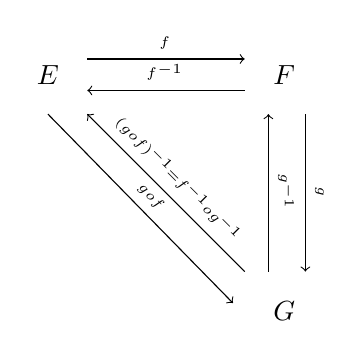
\begin{tikzpicture}
\node (a) at (0,0) {$E$};
\node (b) at (3,0)  {$F$};
\node (c) at (3,-3)  {$G$}; %Corrected node name

%\draw (20) -- (21) -- (22) -- (20) ;
%\draw[->] (0,0) -- (3,0)  ;
\draw[->] (0.5,0.2) -- (2.5,0.2) node[midway,sloped,above] {$_{_f}$};
\draw[->] (2.5,-0.2) -- (0.5,-0.2) node[midway,sloped,above] {$_{_{f^{-1}}}$};

\draw[<-] (2.8,-0.5) -- (2.8,-2.5) node[midway,sloped,above] {$_{_{g^{-1}}}$};
\draw[->] (3.27,-0.5) -- (3.27,-2.5) node[midway,sloped,above] {$_{_{g}}$};
\draw[<-] (0.5,-0.5) -- (2.5,-2.5) node[midway,sloped,above] {$_{_{(gof)^{-1}=f^{-1}og^{-1}}}$};
\draw[->] (0,-0.5) -- (2.35,-2.9) node[midway,sloped,above] {$_{_{gof}}$};
\end{tikzpicture}\newpage

\section{Topolojik Vektör Uzayları}\label{tvu:intro}
Reel yada komplex değerli $\Phi$ cismi üzerinde bir vektör uzayı $E$, $\xi$ de bu vektör uzayında bir topoloji olsun. $E$'deki cebirsel işlemler sürekliyse, $x,y$ için $x+y$ fonksiyonu ve $\lambda, x$ çifti için $\lambda x$ fonksiyonu $E$'de sürekliyse, $\xi$ topolojisi $E$'nin cebirsel yapısıyla \textbf{uyumlu} denir.
\begin{itemize} 
\item[a)]Önce toplama işlemi için,

\begin{align*}
f:E\times E &\longrightarrow E\\
(x,y)&\longmapsto x+y
\end{align*}
verilsin. $f$ fonksiyonunun $E$ kümesinde sürekli olması için, $f(x_0 ,y_0)$'ın $E$'deki her $V$ komşuluğu için, $E\times E$'de $(x_0 ,y_0)$'ın bir $U$ komşuluğu olmalıdır öyle ki, $f(U)\subseteq V$ olsun. $U=U_1 \times U_2$ almak bunun için yeterlidir;\\
 \[f\left(U_1 \times U_2\right)=U_1 + U_2 \subseteq V\]

\item[b)] Skalerle çarpmaya gelirsek,

\begin{align*}
g:\mathbb{R}\times E &\longrightarrow E\\
\left(\lambda, x\right) &\longmapsto \lambda x
\end{align*}
$\lambda_0 x_0$ noktasının $E$'deki her $V$ komşuluğuna karşılık,\\
$\left(\lambda_0 ,x_0\right)$'ın $\mathbb{R}\times E$'de öyle bir komşuluğu vardır ki,\\
\[
\forall\lambda\in\left(\lambda_0 -\varepsilon,\lambda_0 +\varepsilon\right) \text{ ve } x\in U 
\]
komşuluklarını belirlediğimizde, $ g(\lambda,x)=\lambda x\in V$, dolayısıyla $\lambda U\subseteq V$ olur. \\[2pt]

\end{itemize}


$\Phi$ üzerine bir topolojik vektör uzayı, uyumlu bir topolojiyle, $\Phi$ üzerine bir vektör uzayı demektir.\newpage

Şu önermeler süreklilik koşulunun sonuçlarıdır;

\begin{proposition}
Her bir $a\in E$ için, $f:f(x)=x+a$ tasviri $E$'nin kendi üzerine bir homeomorfizmdir. Özel olarak orijin komşuluklarının bir \textbf{baz}ı $\mathscr{U}$ ise, $\mathscr{U}+a$ da $a$ komşuluklarının bir bazıdır.
\end{proposition}

\begin{proof}
Eğer $f(x)=x+a=y$ ise, $f^{-1}(y)=x=y-a$ dır. $f$ ve tersi olan $f^{-1}$ kendi üzerinde sürekli fonksiyonlar olduğu için, $f$ $E$ üzerinde (1-1) tasvirdir. O halde $f$ homeomorfizmdir.\\
$f(x_1)=f(x_2)\Longrightarrow x_1 +\not a=x_2 +\not a,\quad  x_1 =x_2$ (1-1)\\
\[
E\times E\longrightarrow E
\]
\[
\left(x_1 ,x_2\right)\longmapsto x_1 +x_2 
\]
sürekli olduğundan,
\[
E\times \{a\}\longrightarrow E
\]
\[
\left(x,a\right)\longmapsto x+a 
\]
süreklidir. O halde,
\[
E\times \{-a\}\longrightarrow E
\]
\[
\left(x,-a\right)\longmapsto x-a 
\]
ifadesi de süreklidir. Bütün bunlar bir $a$ sabiti için, (1-1), örten ve sürekli bir homeomofizma olduğunu göstermek içindi.\\
$f(x-a)$ noktasının bir komşuluğu $B$ olmak üzere, homeomorfizmden dolayı $f^{-1}(B)$, $(x,-a)$ noktasının içinde bulunduğu bir $U$ komşuluğunun içinde kalır. Bir $x-a$ noktasının yerel bazı $\beta_{x-a}$ ise,  $\beta_{f(x-a)}=\big\{f(U):U\in\beta_{x-a}\big\}$\\
Aynı şekilde $\beta_{x-a}=\big\{f^{-1}(B):B\in\beta_{f(x-a)}\big\}$\\[2pt]
 
Orijin noktası komşuluklarının bir bazı $\mathscr{U}$ ise $E$'nin bütün topolojik yapısı bu baz tarafından belirlenebilir. Bu yüzden genel yapı itibarıyla orijin komşulukları üzerinde çalışıyoruz ve bu sebepten kısaca \emph{komşuluklar} dediğimizde orijin noktasının komşuluklarından bahsediyor olacağız.\\
Eğer $U$ bir komşuluk ise, \emph{(orijin noktasının komşuluğudur bu)}, $U+a$'nın da bir $a$ komşuluğu olması ve $x\in U+a$ olması için g.y.koşul, $x-a\in U$ olmasıdır.\\
Öncelikle biraz daha net görebilmek adına bu son durumu orijin noktasını gözönünde bulundurarak düşünelim. Orijin noktasının bir komşuluğu $U$ ise ve $x\in U$ ise, $x\in U+0$ olacağından, $x-0\in U$ olduğu açıktır. Dolayısıyla $x$ noktamız $0$ komşuluğu ile herhangi bir noktanın \emph{(burada herhangi bir nokta $0$ oluyor)} toplamı kümesi içinde kaldı.
\end{proof}
\begin{remark} $E$ üzerine bir topolojik vektör uzayında tanımlı $x\longmapsto x+a$ tasvirinin sürekliliği, çok önemli bir sonuç ortaya çıkartır. Herhangi bir $a,b\in E$ için, bir $a$ komşuluğu $A$ ise, $b-a+A$ de $b$ noktasının bir komşuluğudur. $a$ noktasının yerel komşuluklar bazına $\mathscr{U}_a$ diyelim. $b$ noktasının herhangi bir komşuluğu ise $B$ olsun. Bir homeomorfizmden bahsettiğimize göre $a-b+B$, $a$'nın bir komşuluğu olacaktır. Bu durumda $a$'nın yerel komşuluklar bazı olan $\mathscr{U}_a$ içerisinde öyle bir eleman bulabiliriz ki, $a$ komşuluğunun içinde kalır. Bu elemana $A$ dersek, $A\subseteq a-b+B$ olacağı açıktır. Bundan dolayı $b-a+A\subseteq B$ olur ki, sol yan \emph{(ve tabi diğer yan da) }bir $b$ komşuluğudur. O halde $b$ komşuluğu, $a$'nın komşuluklar bazı içinde bulunan bir $A$ açık kümesi ile ilgili olarak ortaya çıkar. Homeomorfizmden dolayı sağlanan bu özellik sayesinde, $\{b-a+A:A\in\mathscr{U}_a\}$ kümesi, $b$'nin bir yerel tabanı olduğunu görürüz.

Şunu tekrarlamak faydalı olacaktır; $a$ noktasını $0$ olacak şekilde, orijin noktası olarak seçersek, orijin komşuluklarının bazı $\mathscr{U}$ olmak üzere, $\mathscr{U}+b$ kümesinin, $b$ komşuluklar bazı olduğu ve bu bazın seçtiğimiz farklı bir noktaya \emph{(mesela $0$ noktasına)} bağlı olarak belirlenebileceği görülür.
\end{remark}

\begin{proposition}
$0\neq\alpha\in\Phi$ için $f:f(x)=\alpha x$ tasviri, $E$'nin kendi üzerine bir homeomorfizmasıdır. Özel olarak $U$ bir komşuluk ise, $\forall\alpha\neq 0$ için $\alpha U$ da bir komşuluktur.

\end{proposition}

\begin{proof}
$f(x)=\alpha x=y\Longrightarrow f^{-1}(y)=x=\alpha^{-1}y$ olur.$f(x_1)=f(x_2)\longrightarrow x_1 =x_2$ dir. $\alpha\neq 0$ olduğundan $\not\alpha x_1 =\not\alpha x_2 \quad x_1 = x_2$ olur. (1-1) dir. $y\in E$ alalım. $\alpha\not=0$ olduğundan $\frac{1}{\alpha}y\in E$ olur, o halde $x=\frac{1}{\alpha}y$ alabiliriz. $f(x)=\not\alpha\not{\frac{1}{\alpha}}y=y$, örtendir. O halde bir homeomorfizmadır.

$U$ bir $0$ komşuluğu olduğuna göre, bu komşuluğun altkümeleri arasında öyle bir $S$ açık kümesi vardır ki, $0\in S\subseteq U$ olur. O halde $0$ aynı zamanda bir $\alpha S$ kümesinin de elemanıdır. $\alpha S$ açık bir kümedir ve bundan dolayı $0\in\alpha S\subseteq\alpha U$ olur. Kısaca $U$ açık ve $0$'ın bir komşuluğuysa, $\alpha U$ da açık bir kümedir ve o da bir $0$ komşuluğudur.\newpage
\end{proof}

\begin{proposition}
$\mathscr{U}$ bir komşuluklar bazı ise, $\forall U\in\mathscr{U}$ için;
\begin{itemize}
\item[(i)]$U$ absorbedir,
\item[(ii)]$V+V\subseteq U$ olacak şekilde bir $V\in\mathscr{U}$ vardır,
\item[(iii)]$W\subseteq U$ olacak şekilde  dengeli  bir $W$ komşuluğu vardır.
\end{itemize}
\end{proposition}

\begin{proof} Önerme bize $\forall U\in\mathscr{U}$ ifadesiyle, $0$ noktasının bütün komşulukları için yukarıdakiler geçerli olur demek istiyor.
\begin{itemize}  
\item[(i)] \emph{$0$ noktasının bütün komşulukları absorbe midir?}
$a\in E$ alalım.
\begin{align*}
f:\Phi &\longrightarrow E\\
\alpha&\longmapsto f(\alpha )=\alpha 
\end{align*}
şeklinde bir fonksiyon tanımlayalım. İşimize yarayacağından şöyle bir fonksiyon daha tanımlayalım:
\begin{align*}
g:&\Phi\times E \longrightarrow E\\
&\alpha\times x \longmapsto \alpha x \text{ sürekli ise}\\
&\Phi\times \{a\}\longmapsto \alpha a \text{ kısıtlanmışı da sürekli olur}
\end{align*}
Fonksiyonlardan diğerini de şekil üzerinde gösterecek olursak eğer, bu fonksiyonlar şuna benzer;\\
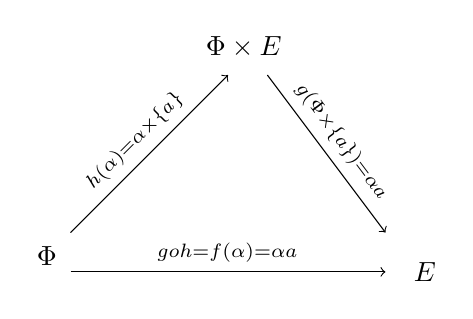
\begin{tikzpicture}
\node (a) at (0.2,0.2) {$\Phi$};
\node (b) at (2.7,2.85)  {$\Phi\times E$};
\node (c) at (5,0)  {$E$}; %Corrected node name

%\draw (20) -- (21) -- (22) -- (20) ;
%\draw[->] (0,0) -- (3,0)  ;
\draw[->] (0.5,0.5) -- (2.5,2.5) node[midway,sloped,above] {$_{h(\alpha)=\alpha\times \{a\}}$};
\draw[->] (3,2.5) -- (4.5,0.5) node[midway,sloped,above] {$_{g\left(\Phi\times \{a\}\right)=\alpha a}$};
\draw[->] (0.5,0) -- (4.5,0) node[midway,sloped,above] {$_{goh=f(\alpha)=\alpha a}$};
\end{tikzpicture}
\newline
$\lambda =0$ için $f(0)=0.a=0\in E$ olduğundan, fonksiyonumuz süreklidir. O halde $E$'de $0$ noktasının bir $U$ komşuluğuna karşılık, $\Phi$ cisminde öyle bir $V$ komşuluğu vardır ki, $\alpha\in V=\{\alpha:|\alpha|\leq\varepsilon\}$ olmak üzere $f$ altında görüntüsü $U$ içerisinde kalır. $\alpha\in V\Longrightarrow \alpha a\in U \Longrightarrow Va\subseteq U$\\
$|\alpha|\leq\varepsilon\Rightarrow\frac{1}{\varepsilon}\leq\frac{1}{|\alpha|}=\mu$ alırsak, $|\mu|\geq\varepsilon^{-1}$ için, $a\in\mu U$ olur.\newpage

\item[(ii)]\emph{$V+V\subseteq U$ olacak şekilde bir $V\in\mathscr{U}$ vardır;}\\
$g(x,y)=x+y$ fonksiyonu $(0,0)$ noktasında süreklidir. $g(0,0)$'ın bir $U$ komşuluğu varsa, ki vardır, $x_1 \in V_1 \text{ ve }x_2 \in V_2$ olacak şekilde, sırasıyla $V_1 ,V_2$ komşulukları vardır. Görüntü kümesinde bulunan bu iki komşuluğun ortak noktaları vardır elbet, bu ortak noktaların oluşturduğu küme bir açık kümedir, o halde bu bir komşuluktur; $V\subseteq V_1\cap V_2$ dersek, $V$ komşuluğunun $\mathscr{U}$ komşuluklar bazı içinde kaldığını görürüz. Bu durumda, $x_1 +x_2 \in U\Rightarrow V+V\subseteq U\subseteq\mathscr{U}$ olur. Biraz daha açıklayıcı olması için,
\[
V+V\subseteq U \Longrightarrow V+V\subseteq \underbrace{\left(V_1 \cap V_2\right)}_{\subseteq V_1}+\underbrace{\left(V_1 \cap V_2\right)}_{\subseteq V_2}\subseteq V_1 +V_2 \subseteq U\subseteq \mathscr{U}
\]
şeklindeki zihin açıcı bir ifadeyle bu şıkkı sonlandıralım.

\item[(iii)] \emph{$W\subseteq U$ olacak şekilde \textbf{dengeli} bir komşuluk vardır.}\\
$W=U$ alarak bu sorunun altından kalkamayız, çünkü $U$ komşuluğu algıladığımızın aksine dengeli olmayabilir. (Neden?) Ama bu $U$ komşuluğu içerisinde kalan dengeli bir \emph{\textbf{komşuluk $=$ açık küme}} mutlaka vardır. 

$h(\lambda ,x)=\lambda x$ alalım.  $\lambda =0, x=0$ noktalarında $h$ fonksiyonu süreklidir. O halde bir $V$ komşuluğu ve $h(\lambda ,x)=\lambda x\in U$ komşuluğu vardır, öyle ki, $x\in V$ ve $\varepsilon>0$, için$|\lambda|\leq\varepsilon$ olsun. Bu durumda $|\lambda|\leq\varepsilon$ için $\lambda V\subseteq U$ olur ve böylece, $|\mu|\geq 1$ için $\varepsilon V\subseteq\mu U$ bulunur. Bundan dolayı, $\varepsilon V\subseteq W=\underset{_{|\mu|\geq 1}}\bigcap\mu U$. \textbf{(Önerme 5)}'ten ötürü $\varepsilon V$ bir komşuluk olduğuna göre, $W$ da bir komşuluktur. Eğer $x\in W$ ve $0<|\lambda|\leq 1$ ise, $|\mu|\geq 1$ olduğunda $x\in\left(\dfrac{\mu}{\lambda}\right)U$ ve bu şekilde $|\lambda|\leq 1$ için $\lambda x\in\mu U$ bulunur. $\lambda x\in W$ olduğundan $W$ dengelidir ve açıkça $U$ içinde yeralır.
\end{itemize}
\end{proof}

\begin{corollary}
Son önermeden şöyle bir sonuç çıkar; her topolojik vektör uzayının bir \textbf{dengeli komşuluklar bazı} vardır. Bu sonucun en önemlisi ve en kullanışlı olanı, \textbf{topolojik vektör uzaylarında orijin noktasının konveks komşuluklar bazı vardır.} Bu tür bir uzaya \textbf{lokal konveks topolojik vektör uzayı} denir. Buna kısaca \textbf{\emph{konveks uzay}} diyeceğiz.\newpage
\end{corollary}

\begin{theorem}
Konveks bir $E$ uzayının orijin noktasının $\mathscr{U}$ komşuluklar bazı, şu özelliklere sahiptir;

\begin{itemize}
\item[(C1)] Eğer $U\in\mathscr{U}$ ve $V\in\mathscr{U}$ ise, $W\subseteq U\cap V$ olacak şekilde bir $W\in\mathscr{U}$ vardır.
\item[(C2)] Eğer $U\in\mathscr{U}$ ve $\alpha\neq 0$ ise, $\alpha U\in\mathscr{U}$
\item[(C3)] Her bir $U\in\mathscr{U}$ mutlak konveks ve absorbedir.
\end{itemize}
Karşıt olarak, bir $E$ vektör uzayının boş olmayan bir $\mathscr{U}$ altkümeler kümesi verilsin, eğer yukarıdaki üç şartı sağlıyorsa,$\mathscr{U}$ bir komşuluklar bazı olacak şekilde, $E$ kümesini \textbf{konveks uzay} yapan bir topoloji vardır.
\end{theorem}
\begin{proof}
$E$ bir konveks uzay olduğundan, tanımdan dolayı, bir konveks komşuluklar bazı vardır. $U$ onlardan biri ise, $U$ içinde kalan konveks kümelerin arakesiti şeklinde, $\underset{_{|\mu|\geq 1}}\bigcap\mu U$ dengeli komşuluğu vardır, konveks kümelerin arakesiti olduğu için konvekstir. (önerme 6). Bundan dolayı mutlak konveks komşulukların bir $\mathscr{V}$ bazı vardır. Bu durumda $\mathscr{U}$ içinde bulunmakta olan bütün $V\in\mathscr{V}$ ve $\alpha V$ kümeleri bir baza ihtiyaç duyar. O halde $\mathscr{U}$ kümeler ailesini oluşturan tüm kümeler için, ki bunlar komşuluktur, $\mathscr{U}$ bir bazdır. Komşuluğun (N2) numaralı özelliğinden \emph{(komşuluklar ailesine ait iki kümenin arakesiti yine bu aileye aittir)} (C1) çıkar. (C2) $\mathscr{U}$ yapısından dolayı gerçeklenir. (C3) de bütün bunların  ve önerme 6 nın bir sonucudur.

Karşıt olarak $\mathscr{U}$ bu teoremin üç özelliğine sahip olsun. $V$ kümesi ise, içinde $\mathscr{U}$'yu barındıran bütün $E$ altkümeleri olsun. Her bir $a\in E$ için $a$ komşuluklarını $\mathscr{V}+a$ ile gösterelim. $V\in \mathscr{V}$ ise, $U\subseteq V$ olacak şekilde $U\in\mathscr{U}$ vardır. $\frac{1}{2}U+a$ komşuluğuna ait her noktanın $V+a$ komşuluğu içinde bulunacağını göstermek gereksiz. 

Toplama işleminin sürekliliğini şöyle gösterelim; $U\in\mathscr{U}$ olmak üzere, $x=a$, $y=b$ olacağını unutmadan, \[x\in\frac{1}{2}U+a \text{ ve } y\in\frac{1}{2}U+b\Rightarrow x+y\in U+a+b\]olur, bu da şu demektir; \emph{$x$, $a$ komşuluğunda ve $y$ de $b$ komşuluğunda ise, $(x+y)$, $a+b$ komşuluğunda kalır.} Matematiksel bir ifadeyle, 
\[
f\Bigg\{\left(\dfrac{1}{2}U+a\right)\times\left(\dfrac{1}{2}U+b\right)\Bigg\}\subset a+b+U
\]
\newpage
$\lambda x$'in sürekliliği için ise; $\lambda=\alpha$, $x=a$ noktaları için öyle bir $\eta$ ve $\delta$ bulalım ki, $|\lambda-\alpha|<\eta$ ve $x\in\delta U+a$ olduğunda $\lambda x-\alpha a\in U$ olsun. \emph{($\lambda x$, $\alpha a$ komşuluğunda kalacak ve buna bağlı olarak $(\lambda x-\alpha a)$, $0$ komşuluğunda kalacak; $\lambda x\in U+\alpha a\Rightarrow\lambda x-\alpha a\in U$)}. Bunun olması için $\lambda$'yı $\left(\alpha -\eta,\alpha+\eta\right)$ şeklindeki bir komşuluktan seçelim, öyle ki, bu komşuluğa bağlı bir $\delta$ için, $x\in\delta U+a$ olsun. \emph{($x-a$, $\delta U$ komşuluğu içinde bulunuyor.)} 
$\mu>0$ olmak üzere, $a$'nın elemanı olacağı bir $\mu U$ komşuluğu bulabiliriz. Bunun için $\mu$ sayısını mutlak konveksliği elde edecek şekilde seçelim. O halde $|\lambda-\alpha|<\eta$ ifadesindeki $\eta$ ile ilgili öyle bir $\mu$ bulalım ki, konvekslik oluşsun;\[0<2\eta<\mu^{-1}\] eşitsizliği bunun için uygun olur.

 (\emph{\textbf{Hatırlatma: $\forall\lambda>0, \mu>0$ ve $\lambda+\mu\leq 1$ için $\lambda A+\mu A\subseteq A$ olması durumunda mutlak konveks idi. $\lambda<1$ ve $\mu<1$ olduğuna dikkat!}})


$0<2\eta<\mu^{-1}$ eşitsizliğinde $\mu^{-1}<1$ olacağından $(\lambda-\alpha)$'nın sürekliliği ve $U$ komşuluğu içinde kalması sağlanırken, mutlak konvekslik de sağlanacaktır.  Aynı şeyi $(x-a)$'nın içinde bulunduğu $\delta U$ komşuluğu için de uyarlamaya çalışırsak, \[0<2\delta<(|\alpha|+\eta)^{-1}\] ifadesinde, eşitsizliğin sol yanının $<1$ olması sebebiyle $\delta$ sayısı kesinlikle $1$'den küçüktür. Bu arada absorbelik durumu için,
\[
|\lambda|<(|\alpha|+\eta)\Rightarrow\lambda\left(\delta U\right)\subseteq(|\alpha|+\eta)\delta U
\] ve
\[
(\lambda-\alpha)<\eta\Rightarrow(\lambda-\alpha)\mu U\subseteq\eta\mu U
\]ifadesi yeterlidir. \emph{(Bir kolaylık; $0$'ın komşulukları absorbedir.)}\\ Son olarak,
\[
\lambda x-\alpha a=\overbracket[0.5pt]{\underbrace{\lambda}_{<|\alpha|+\eta<1}\underbrace{(x-a)}_{\in\delta U}+\underbrace{(\lambda-\alpha)}_{<\eta<1}\underbrace{a}_{\in\mu U}}^{+\lambda a-\lambda a \text{ eklendi }}\in(|\alpha|-\mu)\delta U+\eta\mu U\subseteq U
\]Kanıtımız tamamlanmıştır.

\end{proof}
\newpage
\begin{corollary}
$E$ vektör uzayının mutlak konveks ve absorbe olan altkümelerinden oluşan herhangi bir $\mathscr{V}$ kümesi verilsin. $E$ üzerinde, $\mathscr{V}$'ye ait her kümenin komşuluk olduğu bir cebirsel yapıyla uyumlu olacak şekilde "\textbf{en ince topolojiyi}" bulmak mümkündür. Bu topoloji altında, $E$ bir konveks uzaydır ve buna ait bir komşuluklar bazı,
\[
\varepsilon\bigcap_{_{1\leq i\leq n}}V_i\qquad (\varepsilon>0, V_i \in \mathscr{V})
\]şeklindedir.
\end{corollary}

\begin{proof}
$\varepsilon\bigcap_{_{1\leq i\leq n}}V_i\qquad (\varepsilon>0, V_i \in \mathscr{V})$ formundaki altkümelerden oluşan bir $\mathscr{U}$ kümesi C1-C3 şartlarını sağladığı takdirde, $E$ kümesini bir \textbf{konveks uzay} haline getiren bir $\xi$ topolojisinin komşuluklar bazı olur. $\mathscr{V}$ kümelerinin komşuluk olduğu herhangi bir topolojide, $\mathscr{U}$ kümeleri de komşuluk olmak zorundadır ve bundan dolayı $\xi$ en ince topolojidir.
\end{proof}

Buradan itibaren teoremler ve kanıtlar genel olarak verilecek, ancak bütün bunlar sadece konveks uzaylar üzerinde olacak.

\begin{proposition}
Bir topolojik vektör uzayında konveks, dengeli ve mutlak konveks kümelerin kapanışları da sırasıyla konveks, dengeli ve mutlak konvekstir.
\end{proposition}

\begin{proof}

\end{proof}
$A$ mutlak konveks bir küme olmak üzere, $a\in\overline{A}, b\in\overline{A}$ ve $|\lambda|+|\mu|\leq 1$ olsun. Herhangi bir $U$ komşuluğu için, $V+V\subseteq U$ olacak şekilde bir $V$ dengeli komşuluğu vardır. $x\in A\cap(a+V)$ ve $y\in A\cap(b+V)$ şeklinde $x, y$ noktalarının bulunduğunu düşünelim; bu durumda,
\[
\lambda x+\mu y\in\left(\lambda A+\mu A\right)\cap \left(\lambda a+\mu b+\lambda V+\mu V\right)
\]
\[
\subseteq A\cap \left(\lambda a+\mu b+V+V\right)
\]
\[
\subseteq A\cap \left(\lambda a+\mu b+U\right)
\] 
Bundan dolayı, $\lambda a+\mu b\in\overline{A}$ olur ve böylece $\overline{A}$ kümesinin mutlak konveks olduğu görülür. Dengeli ve konveks kümeler içinde aynı şekilde ispat geçerlidir.

\begin{corollary}
Topolojik bir vektör uzayında \textbf{kapalı, dengeli komşuluklar bazı} vardır. Bir konveks uzay da C1-C3 şartlarını sağlayacak şekilde \textbf{kapalı komşuluklar} bazına sahiptir.
\end{corollary}

\begin{proof}
Bir $\mathscr{U}$ dengeli komşuluklar bazının kapsadığı kümelerin kapanışları da bir komşuluklar bazıdır. \\
$U\in\mathscr{U}$ için, $V+V\subseteq U$ olacak şekilde bir $V\in\mathscr{U}$ komşuluğu vardır. $V$ komşuluğunun kapanışına ait herhangi bir $x$ noktası, $x\in\overline{V}$ alalım. Bu aynı zamanda $x+V$ demektir. (\emph{Hatırlatma: $\overline{V}=\{V\cup V\text{'nin yığılma noktası}\}$}) $x+V$ komşuluğu ile $V$ komşuluğu ortak noktalar içereceğinden, 
\[
x\in \underbrace{V-V}_{0\text{ komşuluğu}}=V+V\subseteq U
\]
Böylece herhangi bir topolojik vektör uzayı, kapalı dengeli komşuluklar bazına sahiptir. Konveks uzay için ise, teroem 2 deki baz olacak şekilde $\mathscr{U}$ alırsak, önerme bize $\mathscr{U}$ kümesine ait bütün komşulukların kapanışlarının mutlak konveks olduğunu söyler.
\end{proof}

\begin{proposition}
$E$ topolojik vektör uzayınının bir komşuluklar bazı $\mathscr{U}$ olsun. Bu durumda $E$'nin \textbf{ayrık/Hausdorff} olması için gerek ve yeter şart;
\[
\bigcap_{U\in\mathscr{U}}U=\{0\}
\]
olmasıdır.
\end{proposition}

\begin{proof}
Eğer $E$ ayrıksa ve $x\neq 0$ ise $x\notin U$ olacak şekilde $U\in\mathscr{U}$ vardır ve böylece $\bigcap_{U\in\mathscr{U}}U=\{0\}$ olur.

Karşıt olarak koşulumuz gerçeklensin ve $x\neq y$ olsun, bu durumda $x-y\notin U$ olacak şekilde bir $U\in\mathscr{U}$ bulunur. O halde, önerme 6 dan dolayı $V+V\subseteq U$ olacak şekilde $V$ dengeli komşuluk bulabilirdik. $x+V$ ve $y+V$ birbiriyle karşılaşmayan ve sırasıyla $x$ ve $y$ noktalarının komşuluğu olsun, $z\in(x+V)\cap(y+V)$ ve buradan
\[
x-y=(z-y)-(z-x)\in V-V=V+V\subseteq U
\]
O halde $E$ ayrıktır.
\end{proof}
\end{document}
